\documentclass[11pt,spanish,a4paper]{article}
% Versión 1.er cuat 2021 Víctor Bettachini < bettachini@df.uba.ar >

% Versión 1.er cuat 2021 Víctor Bettachini < bettachini@df.uba.ar >

\usepackage[T1]{fontenc}
\usepackage[utf8]{inputenc}

\usepackage[spanish, es-tabla]{babel}
\def\spanishoptions{argentina} % Was macht dass?
% \usepackage{babelbib}
% \selectbiblanguage{spanish}
% \addto\shorthandsspanish{\spanishdeactivate{~<>}}

\usepackage{graphicx}
\graphicspath{{./figuras/}}
% \usepackage{float}

\usepackage[arrowdel]{physics}
\newcommand{\pvec}[1]{\vec{#1}\mkern2mu\vphantom{#1}}
% \usepackage{units}
\usepackage[separate-uncertainty=true, multi-part-units=single, locale=FR]{siunitx}
\usepackage{isotope} % $\isotope[A][Z]{X}\to\isotope[A-4][Z-2]{Y}+\isotope[4][2]{\alpha}

\usepackage{tasks}
\usepackage[inline]{enumitem}
% \usepackage{enumerate}

\usepackage{hyperref}

% \usepackage{amsmath}
% \usepackage{amstext}
\usepackage{amssymb}

\usepackage{tikz}
\usepackage{tikz-dimline}
\usetikzlibrary{math}
\usetikzlibrary{arrows.meta}
% \usetikzlibrary{snakes}
% \usetikzlibrary{calc}
\usetikzlibrary{decorations.pathmorphing}
\usetikzlibrary{patterns}

\usepackage[hmargin=1cm,vmargin=1.6cm,nohead]{geometry}
% \voffset-3.5cm
% \hoffset-3cm
% \setlength{\textwidth}{17.5cm}
% \setlength{\textheight}{27cm}

\usepackage{lastpage}
\usepackage{fancyhdr}
\pagestyle{fancyplain}
\fancyhead{}
\fancyfoot{{\tiny \textcopyright DF, FCEyN, UBA}}
\fancyfoot[C]{ {\tiny Actualizado al \today} }
\fancyfoot[RO, LE]{Pág. \thepage/\pageref{LastPage}}
\renewcommand{\headrulewidth}{0pt}
\renewcommand{\footrulewidth}{0pt}


\begin{document}
\begin{center}
\textbf{Física 2} (Físicos) \hfill \textcopyright {\tt DF, FCEyN, UBA}\\
	\textsc{\LARGE Ondas viajeras y estacionarias}
\end{center}

Los ejercicios con (*) son opcionales.

\begin{enumerate}


\subsection*{Parámetros de una onda viajera}

\item Verifique si las siguientes expresiones matemáticas cumplen la ecuación
de las ondas unidimensional.
Grafique las funciones dadas.
\begin{tasks}(3)
	\task $\Psi(x,t)= A \operatorname{e}^{- \lambda ( x - v t)^2 }$
	\task $\Psi(x,t)= \beta ( x + v t )$
	\task $\Psi(x,t)= A \sen{\left[ k (x - v t) \right] }$
	\task $\Psi(x,t)= B \sen^2{ \left( k x -\omega t \right) }$
	\task $\Psi(x,t)= C \cos{(k x)} \sen{ \left( \omega t \right) }$
	\task $\Psi(x,t)= D \operatorname{e}^{i ( k x - \omega t ) }$
\end{tasks}


\item La ecuación de una onda transversal en una cuerda está dada por: $y(x,t) = \SI{0.1}{\metre} \sen{ \left( x \SI{\pi}{\per\metre} - t \SI{4 \pi}{\per\second} \right) }$.
Determine para la onda que se propaga en ella:
\begin{tasks}(2)
	\task amplitud,
	\task frecuencia de vibración, y
	\task velocidad de propagación.
	\task Y en $x = \SI{2}{\metre}$ y $ t = \SI{1}{\second}$, desplazamiento, velocidad y la aceleración de la cuerda.
\end{tasks}


\item La frecuencia angular y número de onda de una onda transversal que se propaga en $\hat{x}$ es $\omega= \SI{10}{\per\second}$ y $k = \SI{100}{\per\metre}$.
En $x_1 = \SI{1}{\kilo\metre}$ y $t_1 = \SI{1}{\second}$ tiene por fase $\phi = \frac{3 \pi}{2}$.
\begin{tasks}
	\task ¿Cuál es la fase en ese mismo punto para $t = 0$?
	\task Considerando que $\phi(x,t) = k x - \omega t+ \phi_0$, ¿cuánto vale $\phi_0$?
	\task ¿A qué velocidad se propaga la onda?
	\task ¿En que tiempo el frente de onda arriba a un $x_2 = 2 x_1$?
\end{tasks}


\item Una cuerda con densidad lineal $\mu = \SI{0.005}{\kilo\gram\over\metre}$ se tensa aplicando una fuerza de \SI{0.25}{\newton}.
El extremo izquierdo se mueve hacia arriba y hacia abajo con un movimiento armónico simple de período \SI{0.5}{\second} y amplitud \SI{0.2}{\metre} mientras se mantiene la tensión constante.
Encontrar:
\begin{enumerate}
	\item La velocidad de la onda generada en la cuerda, la frecuencia y la longitud de onda.
	\item La expresión matemática para el desplazamiento: $y(x,t)$.
	\item La energía cinética media por unidad de longitud, de una partícula del medio.
	\item La energía potencial media por unidad de longitud, de una partícula.
\end{enumerate}


\subsection*{Estacionarias en una cuerda como superposición de viajeras}

\item 
\begin{minipage}[t][2cm]{0.6\textwidth}
Una cuerda de longitud $L = \SI{0.6}{\metre}$, fija en sus dos extremos, oscila en uno de sus modos normales.
La velocidad de propagación de las ondas en dicha cuerda es \(v = \SI{80}{\metre\over\second}\).
En el momento que presenta su máxima amplitud pico a pico esta es de \SI{8}{\milli\metre}.
\end{minipage}
\begin{minipage}[c][1.5cm][t]{0.34\textwidth}
	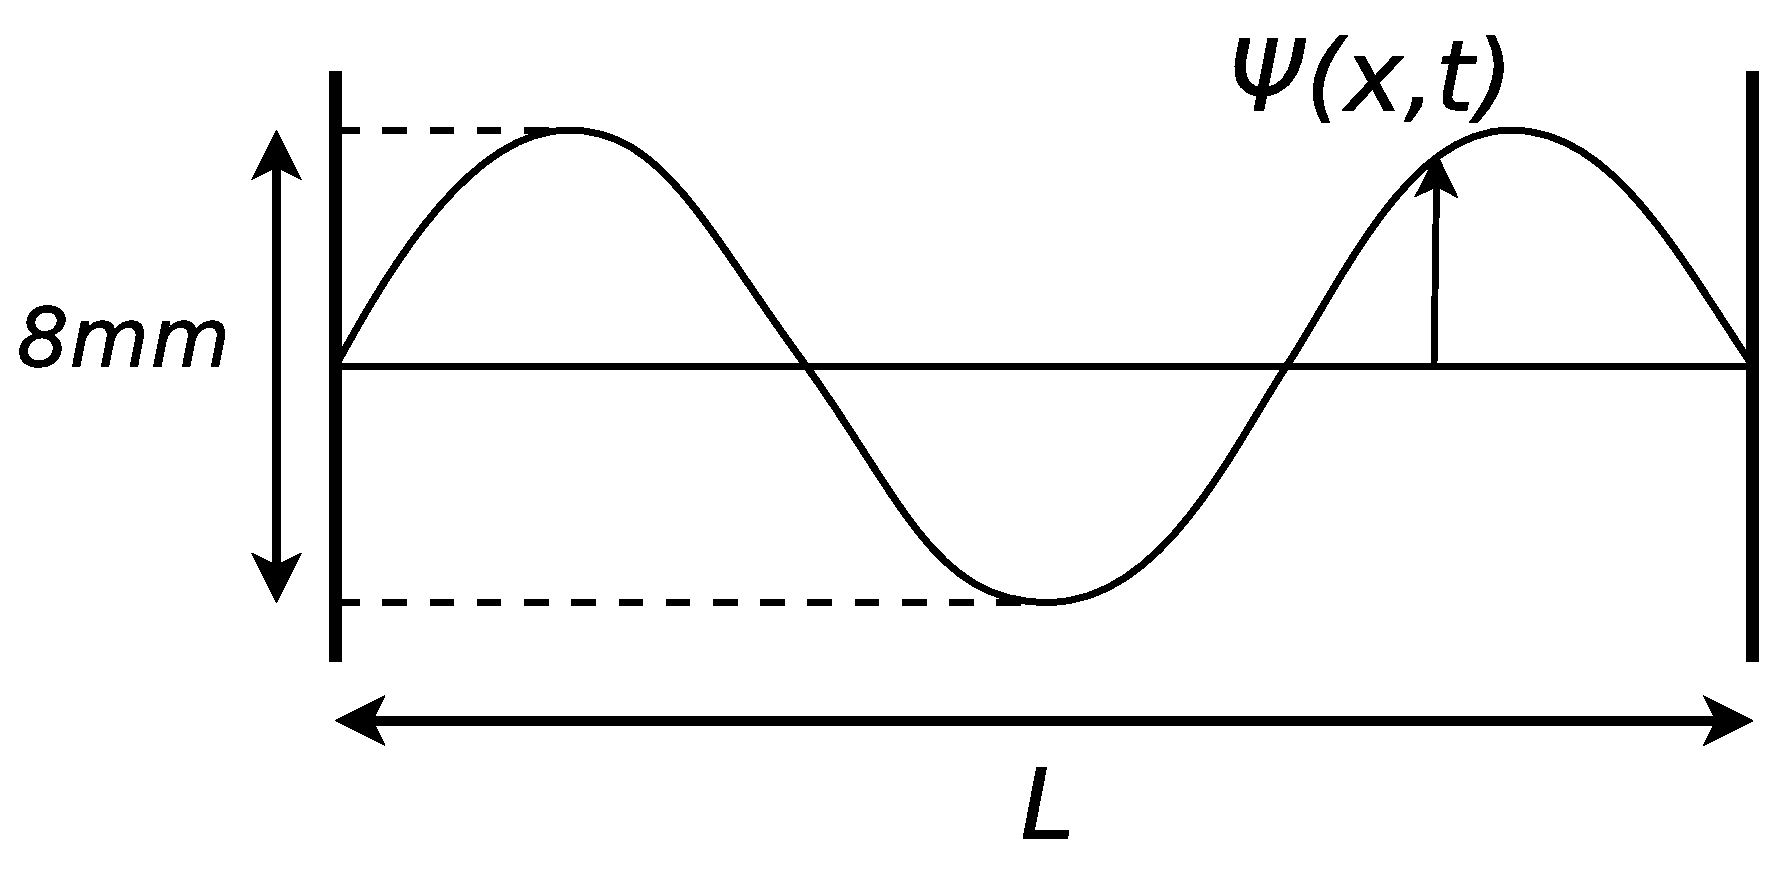
\includegraphics[width=\textwidth]{ej1-32}
\end{minipage}
\begin{enumerate}
	\item Escribir $\Psi(x,t)$, sabiendo que a $\Psi(x,0) = 0\;\forall x$, y que $\dot{\Psi}(L/2,0) > 0$.
	\item Hallar las ondas viajeras $\Psi_{1,2}$ tales que $\Psi(x,t)$ sea una combinación lineal de estas.
\end{enumerate}


\item 
\begin{minipage}[t][2.6cm]{0.6\textwidth}
Una cuerda de longitud $L = \SI{1}{\metre}$, con un extremo fijo y uno libre, oscila en uno de sus modos normales.
La velocidad de propagación de las ondas en dicha cuerda es \(v= \SI{80}{\metre\over\second}\).
En \(t = 0\) presenta su máxima amplitud pico a pico de \SI{8}{\milli\metre}, siendo $\Psi(L,0) > 0$.
\end{minipage}
\begin{minipage}[c][0.4cm][t]{0.34\textwidth}
	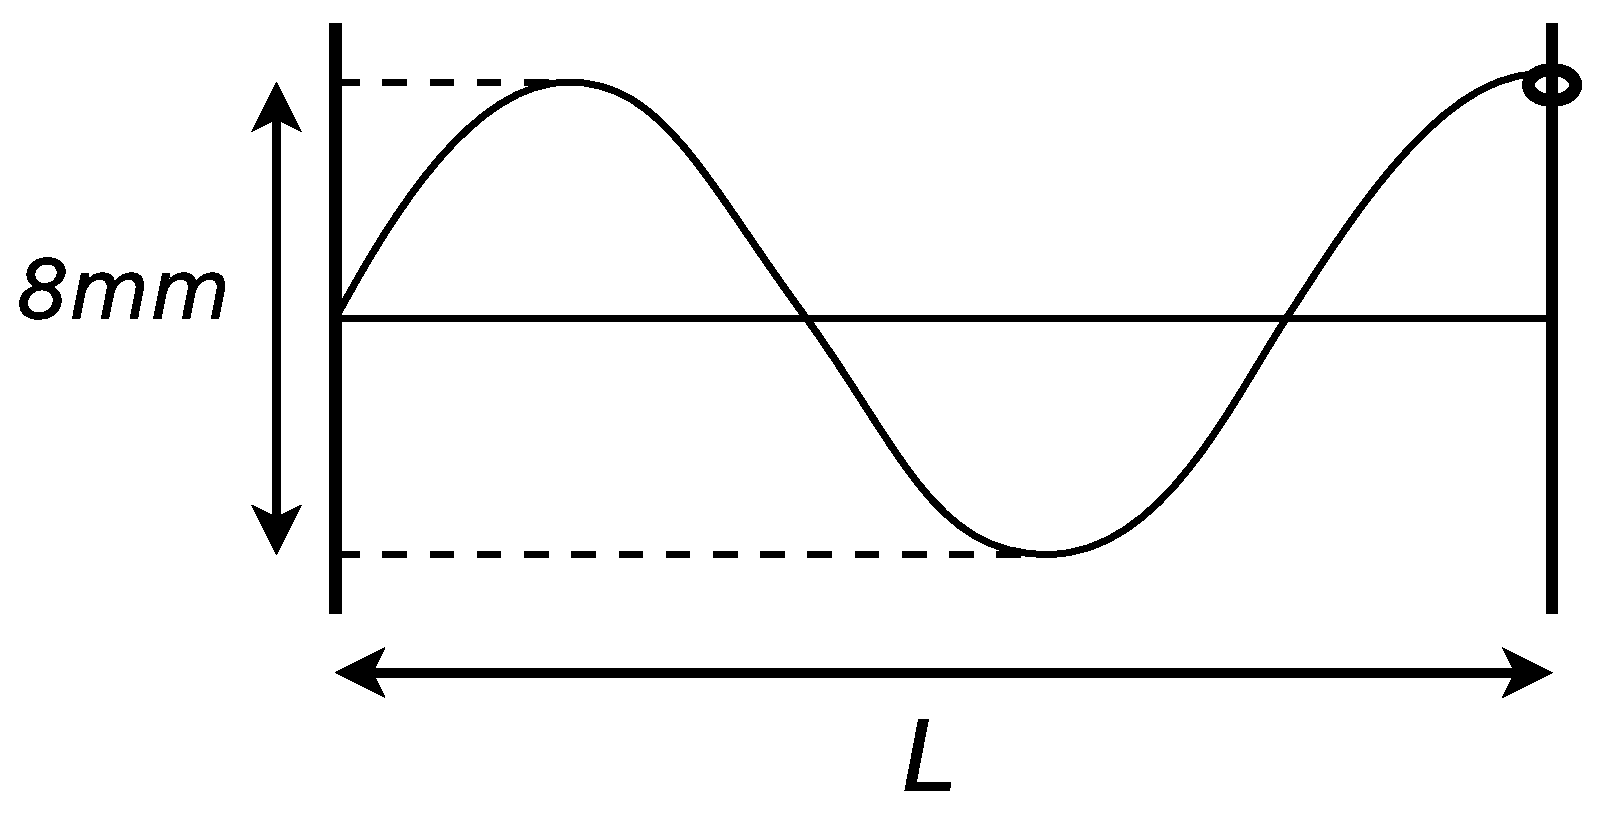
\includegraphics[width=\textwidth]{ej1-33}
\end{minipage}
\begin{enumerate}
	\item Resolver, para esta situación, todo lo pedido en el problema anterior. 
	\item Si ahora la cuerda está oscilando en un modo normal arbitrario $n$, con las mismas condiciones iniciales dadas arriba, repetir (a) (expresar en función de $n$).
\end{enumerate}



\end{enumerate}

\end{document}
